\documentclass[journal=jacsat,manuscript=article]{achemso}

\usepackage{chemformula} % Formula subscripts using \ch{}
\usepackage[T1]{fontenc} % Use modern font encodings
\usepackage{amsmath,amsthm,amssymb}
\usepackage{verbatim}
\usepackage{graphicx}
%\usepackage[dvipsnames]{xcolor}
%\usepackage{SIunits}
% \usepackage[usenames, dvipsnames]{color}
 
 \graphicspath{{figures/}}
\newcommand*\mycommand[1]{\texttt{\emph{#1}}}


\author{Pavel N. Gavryushkin}
\affiliation{Sobolev Institute of Geology and Mineralogy, Siberian Branch of Russian Academy of Sciences, prosp. acad. Koptyuga 3, 630090 Novosibirsk, Russia}
\alsoaffiliation{Novosibirsk State University, Pirogova 2, Novosibirsk 630090, Russia}
\email{gavryushkin@igm.nsc.ru, gavryushkin@g.nsu.ru}

\author{Nursultan Sagatov}
\affiliation{Sobolev Institute of Geology and Mineralogy, Siberian Branch of Russian Academy of Sciences, prosp. acad. Koptyuga 3, 630090 Novosibirsk, Russia}
\alsoaffiliation{Novosibirsk State University, Pirogova 2, Novosibirsk 630090, Russia}

\author{Anatoly Belonoshko}
\affiliation{Department of Physics, AlbaNova University Center, Royal Institute of Technology (KTH), 10691 Stockholm, Sweden}

\author{Maksim V. Banaev}
\affiliation{Novosibirsk State University, Pirogova 2, Novosibirsk 630090, Russia}
\alsoaffiliation{Sobolev Institute of Geology and Mineralogy, Siberian Branch of Russian Academy of Sciences, prosp. acad. Koptyuga 3, 630090 Novosibirsk, Russia}

\author{Konstantin D. Litasov}
\affiliation{Vereshchagin Institute for High Pressure Physics RAS, 108840, Troitsk, Moscow, Russian Federation}



\title {Disordered aragonite---the new high-pressure high-temperature phase of CaCO$_3$}

\keywords{carbonate, density functional theory, melting, experiment, geotherm, mantle, P-T phase diagram}


\begin{document}

\begin{tocentry}
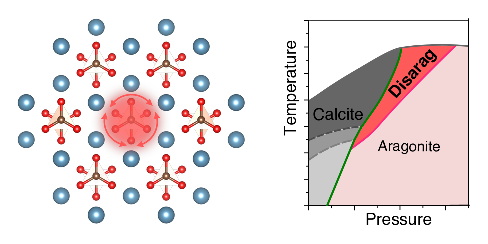
\includegraphics{toc_disarag} \centering
\end{tocentry}


\begin{abstract}
Phases of CaCO$_3$ stabilised at high-pressures and temperatures are the potential agents of the global carbon cycle, transferring oxidised carbon in deep Earth's interiors and thus are of special interest for the Earth sciences. 
Here, we report finding of the new phase, named disarag, which is dynamically disordered aragonite with freely rotating CO$_3$ groups, similar to that in CaCO$_3$-V phase with calcite-like structure. 
Disarag has stability field expanding from 3 to 10 GPa and from 1600 to 2000 K. 
Consideration of twinned structure enlarges this field, decreasing transition temperature from aragonite to disarag on 100--300 K. 
At P-T parameters corresponding to the transition from aragonite to disarag, the marked disappearance of the diffraction peaks is observed in {\it in situ} experiments. 
We show that among known phases of CaCO$_3$ disarag is the best candidate for the explanation of this reconstruction of diffraction pattern. 
Also for the first time, using {\it ab initio} molecular dynamic technique, we determine equilibrium curves between calcite and it's disordered phases CaCO$_3$-IV and CaCO$_3$-V. 
We show that the transition of alkaline-earth carbonates CaCO$_3$, SrCO$_3$, and BaCO$_3$ to the disordered states starts, when the critical angle of CO$_3$ triangle librations about axis perpendicular to the molecular three-fold axis exceeds 45$^{\circ}$. 
Calcite-like structure of CaCO$_3$ is characterised by more intense librations, than aragonite-like structure of this compound and reaches the critical angle at lower temperatures.
As a result, calcite transforms into the disordered state at lower temperatures then aragonite.
\end{abstract}

%%%%%%%%%%%%%%%%%%%%%%%%%%%%%%%%%%%%%%%%%%%%%%%%%%%%%%%%%%%%%%%%%%%%%
%% Start the main part of the manuscript here.
%%%%%%%%%%%%%%%%%%%%%%%%%%%%%%%%%%%%%%%%%%%%%%%%%%%%%%%%%%%%%%%%%%%%%
\section{Introduction}
The recent decade was a revolutionary one in the investigation of CaCO$_3$ phase diagram. 
Lots of new phases were discovered with both experimental and theoretical methods. 
The P-T phase diagram of this simple compound is turned out to be far from simple. It is complicated by the presence of several metastable phases CaCO$_3$-II, III, IIIb, and IV (cc-II, III, IIIb, VI), the joint appearance of several high-pressure phases (CaCO$_3$-VII with aragonite-II \cite{gavr2017_aragII}, and cc-III with cc-IIIb \cite{merlini2014}), the dynamical disordering of calcite (cc-I) structure with the formation of CaCO$_3$-IV (cc-IV) and CaCO$_3$-V (cc-V) phases \cite{ishizawa2013, dove2005}, and amorphisation of the sample at high-pressures and high-temperatures \cite{hou2019_amorph}. 
All set of experimental and theoretical techniques were used for the determination of high-pressure and high-temperature polymorphs, and CaCO$_3$ phase diagram gives several successful examples of cooperative use of {\it ab initio} theoretical methods and experimental techniques for the solution of crystal structures. 
Identification of high-pressure phases CaCO$_3$-VII and aragonite-II \cite{gavr2017_aragII, smith2018}, evidence of tetrahedral coordination of carbon atoms in CaCO$_3$-$P2_1/c-h$ \cite{lobanov2017} and description of the disorder in high-temperature phases cc-IV and cc-IV can be given as examples \cite{dove2005}.

Nevertheless, despite the numerous investigation have been performed, there is still an apparent {\it white spot} on P-T phase diagram of CaCO$_3$, spreading from 3 to 11 GPa and from 800 to 1600 K. 
{\it In situ} X-ray diffraction experiments have revealed marked disappearance of diffraction peaks in this field \cite{suito2001, litasov2017}, with only three peaks left. 
With such a small amount of diffraction information, even simple indexing is problematic. 
The suggested hypothesis assuming the formation of cc-V \cite{suito2001} is inconsistent with available results of quenching experiments \cite{shatskiy2014_feco3}, and no other candidates have been suggested yet. 


In the present work, we perform {\it ab initio} molecular dynamic (MD) simulation of calcite and aragonite and show, that similar to calcite, aragonite adopts disordered state at high temperatures. The disordered aragonite is the good candidate for the phase appeared in the mentioned {\it white spot}.

	%%%
	\paragraph{Crystal structure of aragonite}
	%%%
Crystal structures of calcite and aragonite are similar in the sense, that both them can be presented as the close-packing of Ca-atoms, with CO$_3$ molecular groups occupying octahedral voids \cite{bragg1924}.
In the case of calcite, the packing of Ca atoms is three-layered ({\it fcc}), and CO$_3$ groups are in the centers of the octahedral voids, midway between close-packed (cp) Ca-layers (Figure \ref{str}a).
 In the case of aragonite, the packing of Ca-atoms is two-layered ({\it hcp}), with CO$_3$ groups shifted from the centers of octahedral voids forming the double layer \cite{bragg1924}. 
The upper sublayer is at 1/3 of {\it c'} and the lower one---on 2/3 of {\it c'}, where {\it c'} is the distance between adjacent cp Ca-layers (Figure \ref{str}b). 
In adjacent sublayers, CO$_3$ triangles have opposite orientations, being rotated on 180$^{\circ}$.

\begin{figure}[h]
	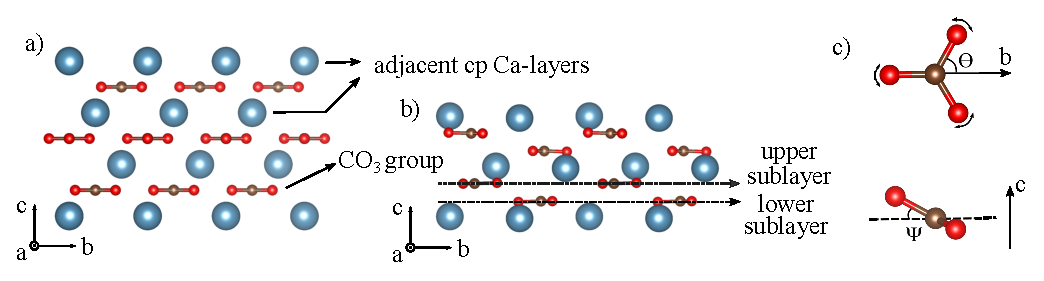
\includegraphics[width=\textwidth]{str}
	\caption{Calcite (a) and aragonite (b) crystal structures along $a$-axis and scheme, showing rotational angle  $\theta$ about three-fold axis of CO$_3$ molecular group and the libration angle $\psi$ about the axis perpendicular to the three-fold axis (c)} \label{str}
\end{figure}


Through the manuscript, we use the aragonite structure in a non-standard $Pmcn$ (\#162) setting. 
In this setting, the comparison of aragonite and calcite structures is more straightforward than in standard $Pnma$ setting, as in both structures $c$-axes are perpendicular to the plane of cp-Ca layer.

Strontianite SrCO$_3$ and witherite BaCO$_3$ at 1 atm have the same structure as aragonite \cite{srco3}. 
These compounds were also used as objects of MD simulations to compare aragonite-like disordered structures with different compositions.


	%%%
	\paragraph{Microstructure of aragonite crystals}
	%%%
Twinning by \{110\} plane is the main microstructural feature of aragonite crystals \cite{marsh1980, suzuki2012, gavr2019_arag}. 
This type of twinning can be produced during crystal growth, or as it was recently shown, mechanically, at crystal splitting \cite{shin2016}. 
In natural aragonite samples, we observed twinning down to the unit-cell size, with the formation of disordered and partially ordered sequences of twinning planes \cite{gavr2019_arag}. 
The ordered sequences of twinning planes are aragonite polytypes, which due to the orthorhombic symmetry, were designated as $O2, O3,\ etc.$ , according to Ramsdell notation \cite{gavr2019_arag}. 

In the present work, to account for the effect of microstructure, we perform MD simulations of not only aragonite but also of $O2$-polytype, which is aragonite twinned by each second \{110\} plane. 
The consideration of the twinned structure is necessary, as powdered samples used in high-pressure experiments are enriched by the twin boundaries produced during grinding.


			%%%%%%%%%%
			\section{Methods}
			%%%%%%%%%%
%	\paragraph{DFT-MD} 	
The total energies and forces were calculated by solving the Schr{\"o}dinger equation based on projector augmented plane-wave  implementation of density functional theory, within the Vienna Ab Initio Simulation Package (VASP) \cite{kresse1999}.
Exchange-correlation effects were treated in the generalised gradient approximation (GGA) with the Perdew-Wang scheme\cite{perdew1992}. 
Pseudo-potentials with $3p^{6}4s^{2}3d^{0.1}$ (Ca), $5s^{2}4d^{0.01}$ (Sr), $s^{1}$ (Ba), $2s^{2}2p^{2}$ (C), and $2s^{2}2p^{4}$ (O) electrons have been used.

We performed finite temperature {\it ab initio} MD simulations to verify the structures and calculate properties. All MD simulations were performed in the isothermal-isobaric {\it NPT} ensemble (N---number of particles, P---pressure, and T---temperature) with Langevin thermostat. The integration of the classical Newton's equations of motion uses the Verlet algorithm, and the ground state search is evaluated within an efficient iterative matrix diagonalisation scheme and a Pulay mixer for each step. A time step for the integration was set to 1 fs. Simulations were performed in the temperature range of 300-2200 K with the step of 100 K. Aragonite  was simulated at pressures of 0, 1.5, 3, 4.5, 6, and 10 GPa, calcite---at 0, 1.5, 3, 4.5, and 6 GPa, while strontianite and witherite---only at 0 GPa.
The integration of Brillouin zone was performed using $\Gamma$-point only. A plane-wave cutoff energy was set to 350 eV. The crystallographic properties were derived from time averages taken over at least 10 ps.

The aragonite, strontianite and witherite were approximated by the supercells, containing 360 atoms, which are $3 \times 3 \times 2$ supercells of the unit cells used. For the calcite, an ortho-hexagonal cell with 480 atoms was used. The supercells of aragonite, strontianite, and witherite were produced based on structural data of De Villeris \cite{srco3}, and supercell of calcite---based on data of Graf \cite{calcite}.


The MD simulations of calcite show that formation of disordered phases cc-IV and cc-V takes place at 1150 and 1300 K, respectively. In experiment, formation of cc-V phase is observed at 1240 K \cite{ishizawa2013}. The close correspondence of experimental and theoretical temperatures shows the correctness of the used technique. 





			%%%%%%%%%%
			\section{Results}
			%%%%%%%%%%
%	\paragraph{QHA} 
In order to determine the stability fields of calcite and aragonite and to estimate the effect of rotational disorder on Gibbs energies of these structures, we will use the results of our calculations of calcite$\leftrightarrow$aragonite equilibrium curve based on quasi harmonic approximation (QHA) and GGA. At present, this work is at the second stage of review in Crystal Growth \& Design journal. Similar results were previously obtained by Ukita and co-authors based on the same QHA approximation but with local density approximation \cite{ukita2016}.

Our results accordingly with the results of Ukita and co-authors \cite{ukita2016}, show that in P-T coordinates the curve, characterising the equilibrium between calcite and aragonite, has the gentle slope at a pressure around 0.6 GPa and temperature around 700 K (Figure \ref{phdia}). 
At temperatures below this point the curve is approximated by the subvertical line, and it became more gentle at higher temperatures.
The presence of the slope on the aragonite$\leftrightarrow$calcite equilibrium curve is in well agreement with the results of numerous experiments and thermodynamic modelling \cite{mirwald1976, redfern2000}. 


The MD simulations of calcite show that at ambient pressure the disordered phases cc-IV and cc-V are formed at 1150 and 1300 K, respectively. 
Simulations in the pressure range of 0--3 GPa shows that the equilibrium curves corresponding to the formation of these phases are nealy parallel with a slightly positive Clapeyron slope in P-T coordinates (Figure \ref{phdia}). 
At pressures above 3 GPa, the slope of cc-I$\leftrightarrow$cc-IV curve became steeper, and as the result at 4.5 GPa the equilibrium curves cc-I$\leftrightarrow$cc-IV and cc-IV$\leftrightarrow$cc-V intersect.
At higher pressures, the transition from cc-I to cc-V proceeds directly, without the formation of intermediate phase cc-IV (Figure \ref{phdia}). 
%However, such a direct transition can be realised only in stability field of aragonite, which is problematic in real experiment.

%	\paragraph{Disarag intro}
Performed MD simulations have shown, that aragonite as well as calcite adopts a disordered state on heating. 
The formation of disordered aragonite, which we have named {\it disarag}, is observed through the whole investigated pressure range up to 10 GPa. 
However, at pressures below 1.5 GPa, it is preceded by the formation of hexagonal aragonite, named hexarag. 
The hexarag is the polymorph of CaCO$_3$ metastable in all P-T range \cite{kawano2009}, it's crystal structure and a possible appearance in experiment were analysed in our mentioned work, submitted to Crystal Growth \& Design journal  \cite{gavr2020_hexar}. 
On further heating, hexarag transforms to the disordered state.
At 0 GPa it takes place at 1500 K.

No hysteresis has been observed for the transition of aragonite to the disordered state. 
The transition occurs at the same temperature, independently whether we increase or decrease the temperature in simulation, at least within the used temperature step of 100 K.

\begin{figure}[H]
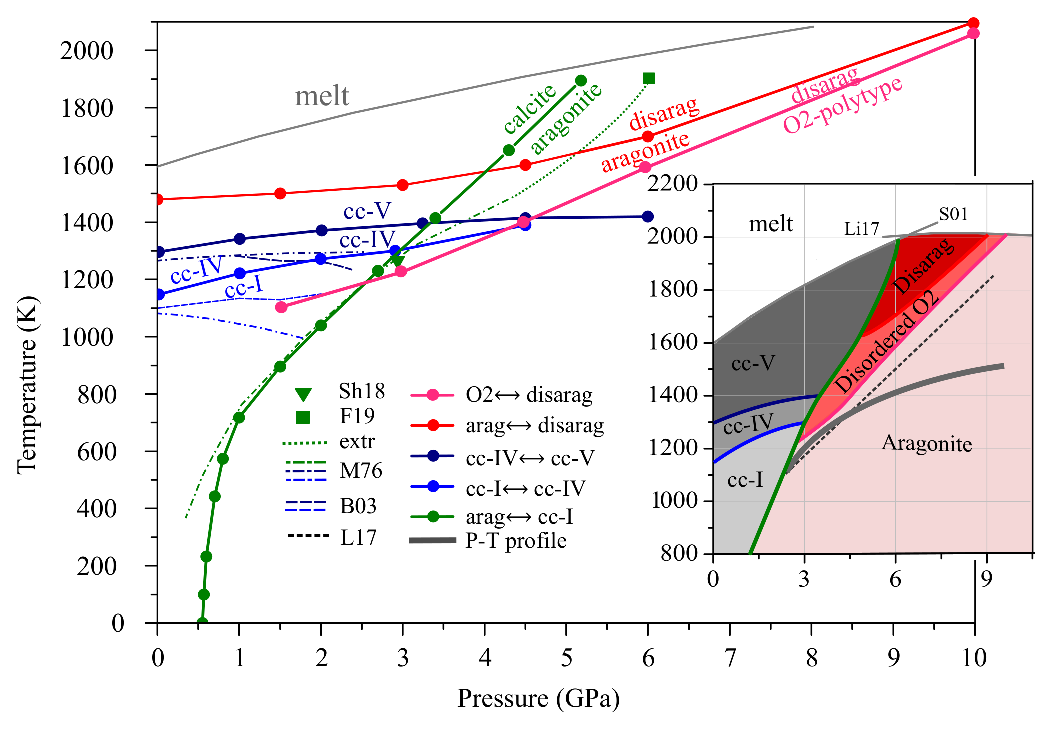
\includegraphics[width=\textwidth]{phdia} \centering
\caption{P-T diagram of CaCO$_3$ with calculated equilibrium curves cc-I$\leftrightarrow$cc-IV, cc-IV$\leftrightarrow$cc-V,  calcite$\leftrightarrow$aragonite, aragonite$\leftrightarrow$disarag, and O2$\leftrightarrow$disarag shown as the solid lines and experimental curves of the phase transitions shown as the dashed and dotted lines; reference data are from: Sh18---\cite{shatskiy2018}, F19---\cite{fedoraeva2019}, M76---\cite{mirwald1976}, B03---\cite{bagdassarov2003}, L17---\cite{litasov2017}, S01-- \cite{suito2001}, and Li17---\cite{li2017}, extr---our extrapolation, P-T profile corresponds to the hot subducting slab \cite{syracuse2010} } \label{phdia}
\end{figure}


At pressure above 1.5 GPa, hexarag is not observed in simulation, and aragonite directly transforms into the disordered state. 
The temperature of disordering is 1500--2100 K for the pressure range of 1.5--10 GPa (Figure \ref{phdia}). 
%As it was mentioned above, in disarag structure CO$_3$ groups freely rotate around the three-fold axis. 
%The description of this rotation and comparison of disordered states in calcite and aragonite will be given below.
The performed simulations of strontianite and witherite show, that these aragonite-like structures also adopt disordered state on heating. 
At 0 GPa, strontianite became disordered at 1400 K, and witherite---at 1300 K. 
Thus, with increasing cation size from Ca$^{2+}$ to Ba$^{2+}$ the temperature of disordering decreases from 1500 K to 1300 K. 


%	\paragraph{V(P) dependence}	
The transition of aragonite into the disordered state is accomplished by the abrupt increase of unit cell volume on $\sim$ 2\% at a pressure of 4.5 GPa (Figure \ref{arag_cell}a).
This value decreases with increasing pressure and at 10 GPa, the volume of disarag is only 0.5\% higher than that of aragonite (Figure \ref{arag_cell}a). 
During transition, the $b$ and $c$ axes increase, while the $a$-axis decreases (Figure \ref{arag_cell}b). 
Our MD simulations show, that transition of calcite into the disordered state is also accomplished by the contraction of the $a$-axis, and expansion of the $b$ and $c$ axes, which is consistent with the experimental results \cite{antao2009} and modelling results obtained with empirical potentials \cite{kawano2009}.

\begin{figure}[H]
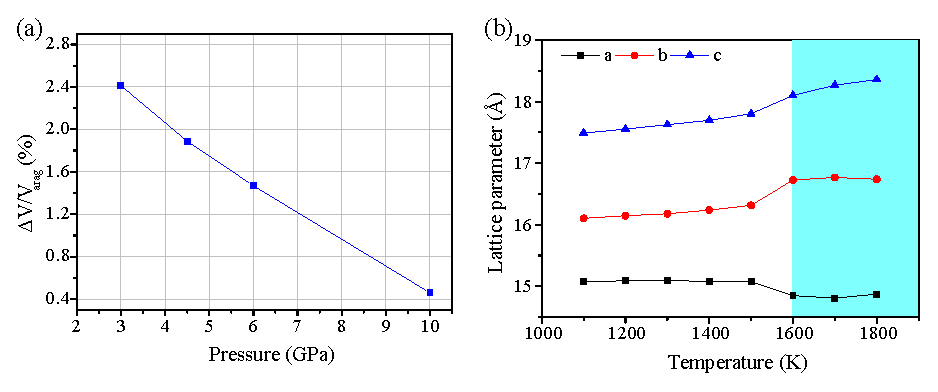
\includegraphics[width=\textwidth]{arag_cell} \centering
\caption{ Ratio of unit cells volumes of aragonite and disarag at aragonite$\leftrightarrow$disarag transformation in the range of 3--10 GPa (a) and dependencies of the cell parameters on temperature for aragonite and disarag (transition marked with the blue band) at 4.5 GPa (b) } \label{arag_cell}
\end{figure}


%	\paragraph{Vibrations around 3-fold axis}
At 300 K and 1.5 GPa, the amplitudes of rotations of CO$_3$ groups about the molecular three-fold axis do not exceed 5$^{\circ}$\ (Figure \ref{rot15}a), whereas with increasing temperature to 1100 K, this value increases to 45$^{\circ}$ (Figure \ref{rot15}b). 
At 1500 K, the amplitude reaches 60$^{\circ}$ and disarag is formed. 
In disarag structure, CO$_3$ triangles rotated on 60$^{\circ}$ and 120$^{\circ}$, making the complete circle around molecular three-fold axis (Figure \ref{rot15}c). 
To reach the disordered state at 1500 K, the simulation run was increased to 30 000 MD-steps, as in a standard simulation with 15 000 steps, disarag was not formed (Figure \ref{rot15}c).
At higher temperatures, 10 000 steps was enough to reach the disordered state.
The distribution function of CO$_3$ triangle orientations in disarag structure is characterised by the presence of six smooth maxima, three of which correspond to the initial equilibrium orientation, and three other---to the anti-orientation rotated on 180$^{\circ}$ (Figure  \ref{distr15}a).

\begin{figure}[H]
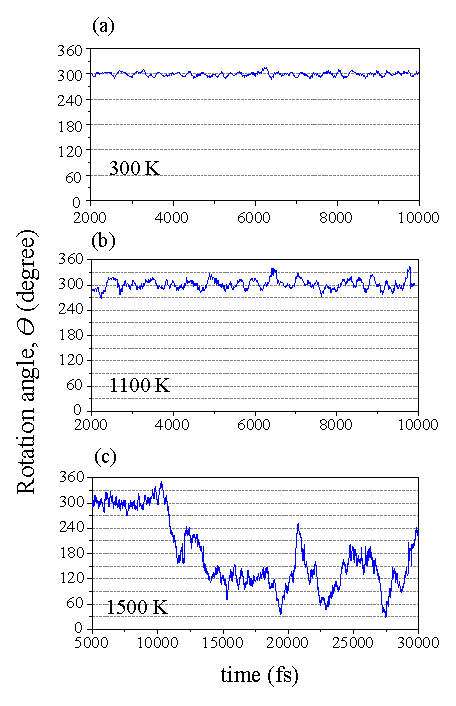
\includegraphics[width=0.5\textwidth]{rot15} \centering
\caption{The dependence of the $\theta$ angle (shown on Figure \ref{str}c) on time for aragonite, at 300, 1100, and 1500 K} \label{rot15}
\end{figure}

\begin{figure}[H]
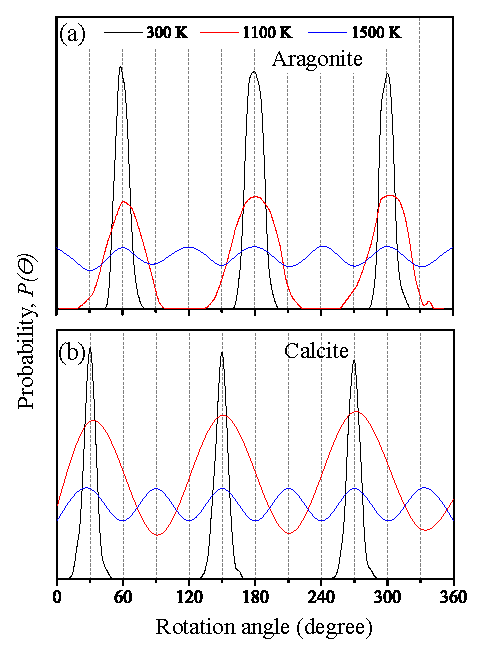
\includegraphics[width=0.5\textwidth]{distr15} \centering
\caption{Probability distribution functions $P(\theta)$ at 1.5 GPa and 300, 1100, and 1500 K for aragonite (a) and calcite (b)} \label{distr15}
\end{figure}

The performed MD simulation of calcite at 1.5 GPa, shows that transitions to the disordered phases cc-IV and cc-V are observed at 1200 K and 1350 K, respectively.
Thus, disordering  of calcite is realised at lower temperatures than that of aragonite (Figure \ref{phdia}). 
The obtained distribution of CO$_3$ triangles orientations for cc-IV and cc-V phases (Figure \ref{distr15}b) is consistent with available experimental \cite{ishizawa2013} and theoretical results \cite{kawano2009}, and it is similar to that of disarag (Figure \ref{distr15}a).


%	\paragraph{Vibrations perpendicular to the 3-fold axis – librations}
The performed simulations have shown, that the movement of the oxygen atoms about the three-fold axis of CO$_3$ group is more complex than simple rotations in plane of CO$_3$ group. 
Such rotations is complicated by the intense librations about the axis orthogonal to the three-fold axis.
Hereafter, the librations about the three-fold axis we will call {\it rotations}, and librations about perpendicular direction---{\it orthogonal librations}
As it will be shown below, orthogonal librations play a crucial role in the transition to the disordered state.

At 300 K and 1.5 GPa, the amplitude of orthogonal librations in aragonite structure reaches 10$^{\circ}$, which is two times higher than amplitudes of rotations at the same P-T conditions.
Heating to 1500 K, increase the maximum amplitude of librations to 45$^{\circ}$ (Figure \ref{libr15}). 
Calcite is characterised by even higher amplitudes of orthogonal librations, with maximum value of 15$^{\circ}$ at 300 K and 1.5 GPa,   and 70$^{\circ}$ at  1500 K, 1.5 GPa (Figure \ref{libr15}).  
The high values of amplitudes of orthogonal librations in calcite and aragonite is consistent with the almost text-book fact of the highly anisotropic thermal expansion of these structures with the high values of thermal expansion coefficients $\alpha_c$  \cite{markgraf1985}.
Noteworthy, that $\alpha_a$ coefficient is negative for calcite \cite{markgraf1985} and positive for aragonite \cite{antao2009, ye2012}, and performed simulations show more intense perpendicular librations for calcite structure.

At 1150 K, when cc-IV transforms to cc-V, the maximum value of amplitudes of orthogonal librations in calcite equals to 45$^{\circ}$. 
The same value of amplitudes is observed for aragonite, when it transforms to disarag, at 1500 K and 1.5 GPa. 
Earlier it was suggested, that flipping of CO$_3$ triangle in anti-orientation can be realised, once the amplitude of perpendicular librations reaches the critical angle \cite{dove2005}.
To check this hypothesis, we determined the values of amplitudes of orthogonal librations at transition to the disordered states for calcite and aragonite at pressures of 0, 1.5, 3, 4.5, and 6 GPa, and also for strontianite and witherite at ambient pressure.
In all cases, we have obtained the same value of 45$^{\circ}$.
This confirms the crucial role of orthogonal librations in transition of carbonates to the disordered states.
Noteworthy, that the value of critical angle does not depend no on the initial structure, no on the chemistry, and it is the same for both calcite and aragonite, and for CaCO$_3$, SrCO$_3$, and BaCO$_3$.

 At 1700 K and 1.5 GPa, the standard deviation of the amplitude of orthogonal librations is 20$^{\circ}$ for aragonite, and it is 33$^{\circ}$ for calcite (Figure \ref{libr15_d}) , with maximum values of 60$^{\circ}$ and 75$^{\circ}$, respectively (Figure \ref{libr15}). 
 At such high values, the average distribution of oxygen atoms of CO$_3$ atomic group actually loses the flat form and became elliptical.
This sufficient deviation from the flat distribution of C--O bond orientations, was earlier highlighted in the work of Cai and-couthors, based on their results of MD simulations with empirical potentials \cite{cai2020}.
Meanwhile, according to the refinements performed based on X-ray diffractions experiments with calcite, the inclination of the orbital of oxygen atoms from the flat form is within $\pm 7.7^\circ$  \cite{ishizawa2013}.
The obtained results show, that suggested from the experimental data umbrella form of the orbital pf oxygen atoms is not characterise the movement of the separate atom, and likely it is the artefact of the initial model used for the refinement.


\begin{figure}[H]
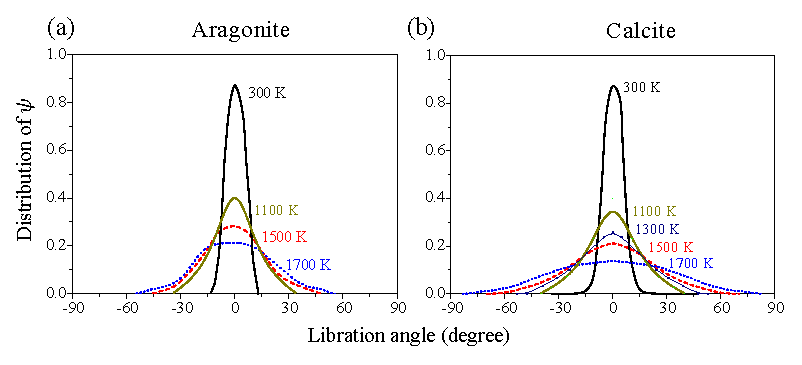
\includegraphics[width=0.95\textwidth]{libr15} \centering
\caption{Probability function for the distribution functions of the amplitudes of orthognoal librations  ($\psi$  angle shown on Figure \ref{str}c) of CO$_3$ triangle for aragonite (a) and calcite (b) at 1.5 GPa and 300, 1100, 1300, 1500, 1700 K} \label{libr15}
\end{figure}

\begin{figure}[H]
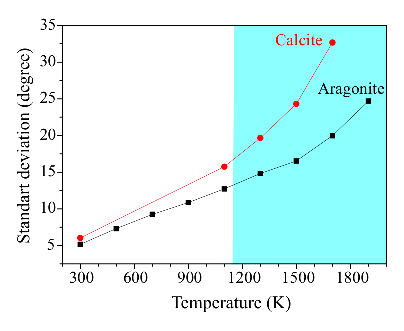
\includegraphics[width=0.5\textwidth]{libr15_d} \centering
\caption{Dependence of the standard deviation of probability function shown on Figure \ref{libr15} on temperature  for aragonite and calcite at 1.5 GPa} \label{libr15_d}
\end{figure}


%	\paragraph{vertical jumping}
Described librations of the CO$_3$ group are also accompanied by the intensive movement of the whole CO$_3$ triangle along the $c$-axis. 
In disarag, the amplitude of such a movement reaches 1/3 distance between cp Ca-layers, which facilitates hoppings of CO$_3$ triangles between adjacent sublayers.
As CO$_3$ groups of adjacent sublayers have opposite orientations, the change of the sublayer is bounded to the change of orientation.
This is illustrated in Figure \ref{z_jump}.
The dependence of $z$-coordinate on time (Figure \ref{z_jump}a)  shows that in the range of 5000--15000 MD steps, the CO$_3$ triangle stays within the same sublayer.
The average coordinate of {\it triangle1} is nearly 2/3 and that of {\it triangle2}---nearly 1/3.
After 15 000 MD-steps, z-coordinate of {\it triangle1} abruptly drops to 1/3, while that of {\it triangle2} abruptly increases to 2/3.
This mean, that {\it triangle1} have hopped from the upper sublayer to the lower sublayer, and {\it triangle2}---in the opposite direction.
The change of the sublayer is accompanied by the rotation of the CO$_3$ group on 60$^{\circ}$, ac can be seen from the dependence of rotation angle on time (Figure \ref{z_jump}b). 
Within the new sublayer, CO$_3$ triangle stays in the range of 15000--25000 steps, and then the next hop between sublayers takes place (Figure \ref{z_jump}a).
This hop is also accompanied by the rotation on 60$^{\circ}$ (Figure \ref{z_jump}a).
Thus, disarag structure presents the new type of disorder related to the position of CO$_3$ group along the $c$-axis. 
This type of disorder is strictly bound to the disorder of the orientation of CO$_3$ group.
In the MD simulation of witherite BaCO$_3$, the transition to the hexagonal symmetry have been noticed by Cai and co-authors \cite{cai2020}.
Asuming rotational disorder of the carbonate group and it's average position midway between cp-layers, the symmetry of the disarag structure will be also hexagonal the same as that of NiAs.


\begin{figure}[H]
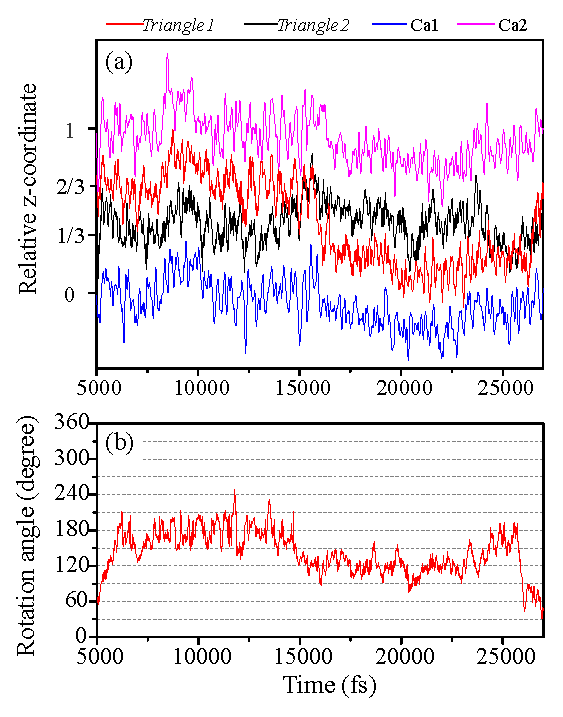
\includegraphics[width=0.55\textwidth]{z_jump} \centering
\caption{The dependence of relative $z$-coordinate on time for two Ca atoms (Ca1 and Ca2) lying in the adjacent cp-layers and for two carbon atoms, belonging to CO$_3$ groups called {\it triangle1} and {\it triangle2} (a) and the dependence of {\it triangle1} orientation on time (b); pressure equals to 4.5 GPa, temperature to--1600 K} \label{z_jump}
\end{figure}



%	\paragraph{The effect of twinning}
To account for the effect of defects on the temperature of aragonite disordering, the MD simulations of the aragonite structure twinned by each second (110) plane have been performed.
As it was mentioned in the Introduction, aragonite structure twinned in such a manner corresponds to the so-called {\it O2-polytype} \cite{gavr2019_arag}.
In this case, $O2$-polytype is the theoretical approximation of the real structure with the disordered sequence of twinned boundaries, observed in experiments \cite{gavr2019_arag}.
The simulation of the polytypes with the less density of twin boundaries and even more the structure with the disordered sequences of twin boundaries is too expansive in sense of computer resources.

Performed simulations have shown, that as well as aragonite, O2-polytype became disordered at high temperatures. 
The temperature of disordergin is lower than that of aragonite.
At pressures below 3 GPa, the difference in transition temperatures for twinned (O2-polytype) and normal (aragonite) structures is around 400 K (Figure \ref{phdia}). 
The difference decreases with pressure and at 9 GPa it is just 100 K.


			%%%%%%%%%%
			\section{Discussion \& Conclusions}
			%%%%%%%%%%

%	\paragraph{formation of disordered calcite} 
The obtained results, describing equilibrium curves between calcite and its disordered forms cc-IV and cc-V, show that the curves corresponding to the transitions cc-I $\leftrightarrow$ cc-IV and cc-IV $\leftrightarrow$ cc-V are almost parallel within P-T stability field of calcite. 
This is in full agreement with experimental data on cc-IV $\to$ cc-V transition \cite{bagdassarov2003, redfern1989, mirwald1976}, shown on Figure \ref{phdia}. 
A comparison of theoretical and experimental results on cc-I $\to$ cc-IV transition is not so straightforward, as the appearance of the intermediate phase cc-IV phase on the heating history of the sample and maybe on some other factors.
Based on differential thermal analysis experiments, Mirwald suggests the negative Clapeyron slope for the equilibrium curve cc-I $\leftrightarrow$ cc-IV  \cite{mirwald1976}. 
This assumes an expansion of the cc-IV stability field with pressure increasing (Figure \ref{phdia}).
However, the results of Mirwald depend on the direction, in which the phase boundary is crossed over.
In case, when the boundary is crossed in the direction of cooling, the Clapeyron slope is close to zero, which is consistent with our results. 
Similar difficulties were revealed by Bagdassarov and co-authors in their measurements of electrical impedance  \cite{bagdassarov2003}.
According to these results, the phase boundary is subhorizontal with a slightly positive slope (Figure \ref{phdia}). 
Thus, the stability field of cc-IV not expands but contracts with pressure, and at a pressure above 3 GPa this phase disappear, which is reproduced in our simulations. 
According to our results, the triple point of cc-I, cc-IV, and cc-V co-existence is located at 5 GPa and 1400 K.
At pressures above this value, cc-IV does not form, and cc-I directly transforms into cc-V on heating.
However, this can not be observed in experiments, as calcite is metastable at such high pressures.


%	\paragraph{aragonite to calcite transformation}
For {\it ab initio} determination of the stability field of disarag the comparison of Gibbs energies of disordered phases of calcite (in ordered and disordered forms) and disarag is necessary.
As {\it ab initio} calculation of the entropy of dynamically disordered phase is the complex task, we will use the results of quenching experiments for determination of equilibrium curve between calcite and aragonite.
In this case, we assume that disordered aragonite is quenched in aragonite and disordered calcite---in calcite.
The results of our unpublished calculations of calcite$\leftrightarrow$ equilibrium curve, which we have mentioned above, will be used for comparison.

The calculated equilibrium curve of calcite $\leftrightarrow$ aragonite transition obtained within QHA is in remarkable agreement with the results of quenching laboratory experiments \cite{shatskiy2018, fedoraeva2019}, at temperatures where disordering does not take place, i.e. before formation of cc-IV (Figure \ref{phdia}). 
%For comparison we use the results of quenching experiments, in which temperature of aragonite to calcite transformation was determined with the precision of 25 C$^{\circ}$ at 3 GPa \cite{shatskiy2018} and  with the precision of 50 C$^{\circ}$ at 6 GPa \cite{fedoraeva2019}.
After formation of cc-IV, the theoretical results based on QHA, which does not account for the rotation of CO$_3$ triangles, start to deviate from the experimental ones. 
The disordering of calcite structure decreases its Gibbs energy, thus stabilising calcite against aragonite. 
This results in expansion of calcite stability field in comparison with stability field determined with QHA.
The aragonite disordering partially or completely compensates this energy difference, and above 1600 K experimental curve of calcite $\leftrightarrow$ aragonite equilibrium is parallel to the theoretical one, as it is shown on Figure \ref{phdia}.

%	\paragraph{stability field of disarag}
The found disordered phase of aragonite has the distinct stability field on P-T diagram (Figure \ref{phdia}). 
In the pressure range of 3--10 GPa, formation of disarag precedes melting on 0--500 K. 
The transition from aragonite to disarag occurs at temperatures at least 300 K higher than the temperatures of the slab subducting in the upper mantle.
The curve corresponding to the transition from O2-polytype to disarag is almost touch the hot geotherm of the subducting slab at 3.5 GPa, which corresponds to the depth of nearly 110 km \cite{syracuse2010}.
This assumes possibility of disarag formation at these depths, although in the narrow pressure range.

%	\paragraph{in situ experiments}
Assuming that disarag is quenched in aragonite, as well as disordered calcite is quenched in calcite \cite{ishizawa2013}, it can be concluded, that formation of disarag is consistent with available results of quenching experiments.
However, only {\it in situ} experiments can approve the formation of disarag. 
Results of these experiments consistently show transition to the new phase at P-T parameters, where aragonite transforms to disarag in our simulations (Figure \ref{phdia}). 
The temperature difference between transition observed in experiments  \cite{litasov2017, suito2001} and in our simulations is just 200 K (above 6 GPa) for normal aragonite, and 100 K---for twinned aragonite.
However the structure of the phase obtained in experiment is debated.
This is partially, due to the mentioned lack of diffraction information.
The hypotheses, suggested cc-V \cite{suito2001}, some disordered phase \cite{litasov2017} and amorphous phase \cite{hou2019_amorph} have been proposed.
Appearance of cc-V phase at these P-T parameters is inconsistent with results of quenching experiments (Figure \ref{phdia}).
The unique character of amorphisation observed at high pressures and temperatures and absence of amorphisation in the other experiments performed at the same P-T parameters \cite{litasov2017,suito2001} states the question about the thermodynamic stability of the amorphous phase and  reproducibility of this experiment.
Summarising, we conclude that among known phases of CaCO$_3$, disarag is the best candidate for the explanation of structural changes observed in experiment.
However, the appearance of the other strusture in ordered or disordered form can not be excluded.


%As it was mentioned in the Introduction, the reliable indexing the X-ray diffraction pattern obtained in experiment, which contains only three diffraction peaks, is problematic.
%However, the lack of diffraction peaks itself is consistent with the disordered character of the formed phase.
%Among known phases of CaCO$_3$, the found structure of disordered aragonite is likely the only candidate  for the high-temperature phase, which formation is consistent with available experimental results.

%Recently, the amorphisation of aragonite taking place on heating at 4--8 GPa was found. This unique case of amorphisation on heating have yet been observed only for CaCO$_3$ and it is not known for other coompounds. 
%For aragonite, the amorphisation was observed only in one experiment performed in Paris-Edinburgh press \cite{hou2019_amorph} and it was not observed in the experiments with multi-anvill apparatus \cite{litasov2017, suito2001}. 
%As amorphisation is observed at nearly the same parameters as found aragonite disordering, it can be suggested that in some cases intense vibrations in disordered phase lead to the amorphisation of the sample. 

In conclusion, we would like to highlight, that earlier only calcite-type disordered structures were known. 
These are CaCO$_3$-IV, CaCO$_3$-V, rhombohedral SrCO$_3$, rhombohedral BaCO$_3$, and cubic BaCO$_3$.
Here, we have shown that aragonite also became disordered, although at high pressures.
Even at ambient pressure, solution of disordered structures is nontrivial task, as the example of disordered calcite has shown.
This task became sufficiently more complex at conditions of high-pressures, where diffraction data are of intrinsically low quality.
In this case, the application of MD simulation technique became absolutely necessary step of the successful determination and characterisation of the structure.

\begin{acknowledgement}
The study was funded by RFBR according to the research project \#18-35-20047. 
Part of the work on simulation of disordered phase of calcite was also supported by the state assignment project of IGM SB RAS. 
ABB is supported by the Swedish Scientific Council research grant 'Mineral physics of the Earth Core'. 
The computations were performed using resources provided by SNIC through National Supercomputer Center at Link\"{o}ping Technical University (Sweden) and by Novosibirsk State University Supercomputer Center (Russia).
\end{acknowledgement}

%%%%%%%%%%%%%%%%%%%%%%%%%%%%%%%%%%%%%%%%%%%%%%%%%%%%%%%%%%%%%%%%%%%%%
%% The appropriate \bibliography command should be placed here.
%% Notice that the class file automatically sets \bibliographystyle
%% and also names the section correctly.
%%%%%%%%%%%%%%%%%%%%%%%%%%%%%%%%%%%%%%%%%%%%%%%%%%%%%%%%%%%%%%%%%%%%%
\bibliography{Gavr_scilib}
%\bibliography{achemso-demo}

\end{document}
